%\documentclass[t,handout]{beamer}
\documentclass{beamer}


\usepackage[utf8]{inputenc}
\usepackage[english]{babel}
%\usepackage[tight]{subfigure}
\usepackage{graphicx}
\usepackage{color}
\usepackage{url}
% \usepackage{listings}
%\usepackage[alf]{abntcite}


%\usetheme{Frankfurt} %LEGAL     !!!
% \usetheme{Madrid}     %LEGAL/L%IMPO/COM CAIXA     (sem barra de desenvolvimento)

% \usetheme{Antibes} %NAO
%\usetheme{Berlin} %PODE SER...     (BARRA DE DESENVOLVIMANTO)
% \usetheme{Berkeley}     %FEIO
% \usetheme{Boadilla} %TUDO BRANCO...
% \usetheme{Copenhagen}     %NAO
% \usetheme{Darmstadt} %LEGAL!     !!!
 \usetheme{Dresden}     %LEGAL/LIMPO/SEM CAIXA     (sem caixa fica ruim...)

% \usetheme{Goettingen}     %FEIO DEMAIS!
%\usetheme{Ilmenau} %LEGAL (forte candidato)
% \usetheme{JuanLesPins} %BACANA
% \usetheme{Luebeck}     %FEIO

% \usetheme{Malmoe}     %FEIO
% \usetheme{Warsaw} %NAO...
% \usetheme{Seattle}
% \usetheme{CambridgeUS}
% \usetheme{Singapore}

% \usecolortheme[RGB={130,35,150}]{structure}
% \usecolortheme[RGB={33,33,94}]{structure}
\usecolortheme[RGB={134,153,188}]{structure}
\setbeamertemplate{footline}[frame number]
\setbeamertemplate{navigation symbols}{}

%Hide subsections on teable of contents
%\hypersetup{bookmarksopen=true,bookmarksopenlevel=4}
%\setcounter{tocdepth}{2}



\author[]{\textbf{Spc. Antonio Esteves} and Dr. Leonardo M. Medeiros}

%\date{\today}
\date{22/08/2018}
\institute[]{Federal Institute of Alagoas - BRAZIL
}
\title{A predictive analysis approach using linear regression to estimate software effort}
%\logo{\includegraphics[width=0.2\linewidth]{img/logo.png}}
\subtitle{\textbf{ERBASE 2018}}

\begin{document}

\begin{frame}
  \titlepage
\end{frame}

{\frame{
\frametitle{Summary}
\tableofcontents
}
}

\section{Motivation}
\subsection{}
\begin{frame}{Software development effort and productivity}
	\begin{block}{}
	Nowadays, predict software development time and budget is a real challenge with economic and scientific relevancy. So, the accuracy of a predict software estimation model has a vital role in software development and effort prediction estimation is one of the critical tasks required for developing software.
	\end{block}

  \begin{block}{}
  	This work presents regression and machine learning techniques to predict software effort estimation, through data from existing projects.
  \end{block} 
\end{frame}

\begin{frame}{Effort Estimation}
  \begin{block}{}
%   In software project management, effort estimation is the process of developing an approximation of the monetary and temporal resources needed to complete project activities. The software effort estimation can be seen as a small size project which needs to be carefully planed, managed and followed up.
  \end{block}  
	\begin{block}{}
	\centering
    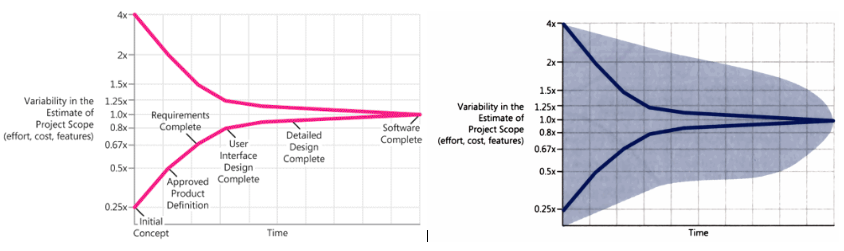
\includegraphics[height=4.65cm,width=4.6 in]{img/uncertainty_cone.png}\hspace*{\fill}
	\end{block}
\end{frame}

\begin{frame}{Effort Estimation}
  \begin{block}{}
    
  
One of the fundamental issues in a software project is to know how much effort will be spent in working hours or budget before starts the software development. Actually, companies uses insufficient background of metrics in the area of software estimation.
	\end{block}
\end{frame}

\begin{frame}{Learning-oriented models}
  \begin{block}{}
The Learning-oriented models attempts to automate the estimation process by building autonomous models that can learn from previous estimations experiences. These models do not rely on assumptions and are capable of learning incrementally as new data are provided over time.
  \end{block}
\end{frame}

\begin{frame}{AI-based Predictive Models}
  \begin{block}{}
AI-based predictive models can be a useful tool with an accurate degree that helps on the prediction of software effort based on historical data from software development metrics.
	\end{block}
     \begin{block}{}
In this study, we built a software effort estimation model to predict this effort using a Linear Regression model.
  	\end{block} 
\end{frame}

\begin{frame}{Data Collection}
	\begin{block}{}
	To perform this study we used Desharnais dataset from the PROMISE software engineer repository. This dataset consists of 81 software projects from a Canadian software house collected by J. M. Desharnais.
	\end{block}
\end{frame}


\begin{frame}{Features definition to Desharnais dataset}
	\begin{block}{}
      \begin{table}[H]
      \centering
      \label{tab:datasetFeaturesTable1}
      \smallskip
      \resizebox{\columnwidth}{!}{%
      \begin{tabular}{|l|l|}
      \hline
      \textbf{Feature} & \textbf{Description}\\[0.5ex]
      \hline
      &\\[-2ex]
      Project & Project ID which starts by 1 and ends by 81\\[0.5ex]
      \hline
      &\\[-2ex]
      TeamExp & Team experience measured in years\\[0.5ex]
      \hline
      &\\[-2ex]
      Manager Exp & Manager experience measured in years\\[0.5ex]
      \hline
      &\\[-2ex]
      YearEnd & Year the project ended\\[0.5ex]
      \hline
      &\\[-2ex]
      Length & Duration of the project in months\\[0.5ex]
      \hline
      &\\[-2ex]
      Effort & ActualEffort is measured in person-hours\\[0.5ex]
      \hline
      &\\[-2ex]
      Transactions & Transactions is a count of basic logical transactions in the system\\[0.5ex]
      \hline
      &\\[-2ex]
      Entities & Entities is the number of entities in the systems data model\\[0.5ex]
      \hline
      &\\[-2ex]
      PointsAdj & Size of the project measured in unadjusted PointsAdj
      function points.\\[0.5ex]
      \hline
      &\\[-2ex]
      PointsNonAdjust & Size of the project measured in adjusted function points.\\[0.5ex]
      \hline
      &\\[-2ex]
      Language & Type of language used in the project expressed as 1, 2 or 3.\\[0.5ex]
      \hline
      \end{tabular}}
      \end{table}
	\end{block}
\end{frame}

\section{Fundamentals}
\subsection{}
\begin{frame}{Linear Regression}
	\begin{block}{}
		Regression analysis aims to verify the existence of a functional relationship between a variable with one or more variables, obtaining an equation that explains the variation of the dependent variable Y, by the variation of the levels of the independent
variables.
	\end{block}
\end{frame}

\begin{frame}{K-Nearest Neighbors Regression}
	\begin{block}{}
		\begin{itemize}[<+->]
			\item K-Nearest Neighbor Regression is a simple algorithm that stores all available cases and predict the numerical target based on a similarity measure (e.g., distance functions);
            \item  The input consists of the K closest training examples in the feature space;
            \item It’s been used in a statistical estimation and pattern recognition as non-parametric technique classifying correctly unknown cases calculating euclidean distance between data points;
		\end{itemize}
	\end{block}
\end{frame}

\begin{frame}{K-Nearest Neighbors Choice}
	\begin{block}{}
			Our choice by \textit{K-Nearest Neighbor} Regression was motivated by the absence of a detailed explanation about how effort attribute value is calculated on Desharnais dataset;
	\end{block}
\end{frame}

\section{Effort Estimation}
\subsection{}
\begin{frame}{Feature Selection}
	\begin{block}{}
	To address Desharnais dataset the correlations between attributes and software effort were analyzed. The correlation between two variables is a measure of how well the variables are related.
	\end{block}
\end{frame}


\begin{frame}{Pearson Correlation}
	\begin{block}{}
	The most common measure of correlation in statistics is the Pearson Correlation which shows the linear Relationship between two variables. Pearson correlation coefficient (PCC) is a statistical metric that measures the strength and direction of a linear relationship between two random variables.
	\end{block}
\end{frame}

\begin{frame}{Pearson's Correlation Matrix}
		 \begin{block}{}
			\begin{center}
				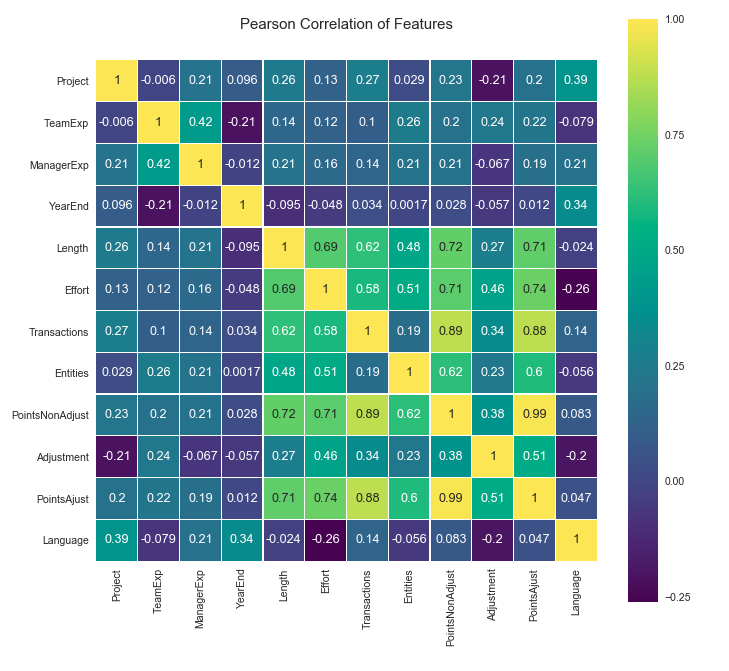
\includegraphics[height=2.6 in]{img/pearsons_correlation_matrix.png}
			\end{center}
		 \end{block}
\end{frame}

\begin{frame}{Pearson's Correlation Matrix}
		 \begin{block}{}
			\begin{center}
				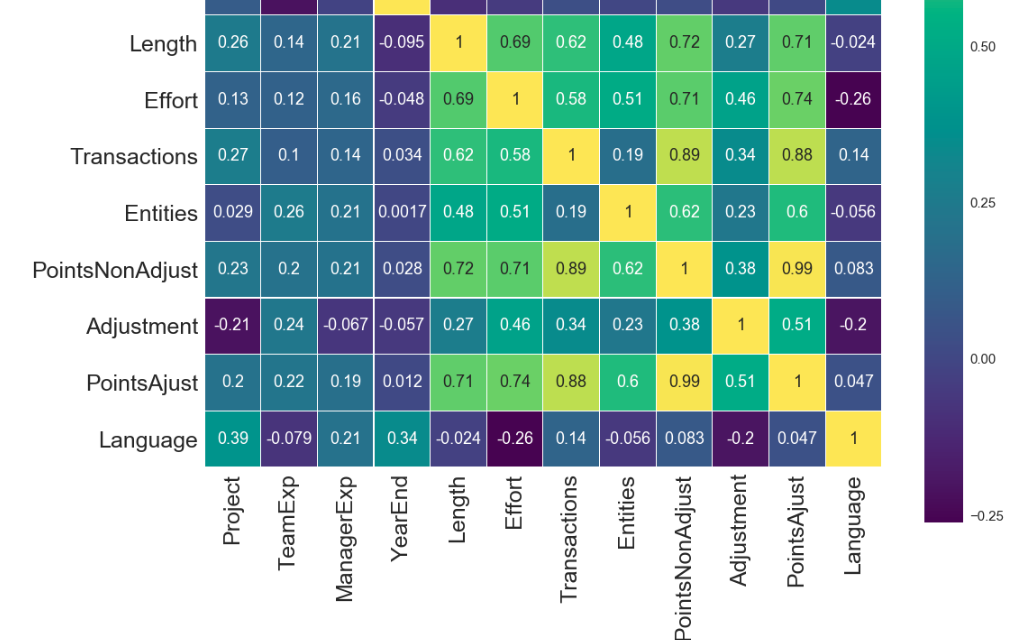
\includegraphics[height=2.6 in]{img/pearsons_correlation_matrix_sliced.png}
			\end{center}
		 \end{block}
\end{frame}

\begin{frame}{Model Construction}
	\begin{block}{}
		\begin{itemize}[<+->]
            \item \textit{Linear Regression} and \textit{K-Nearest Neighbors Regression};
			\item Linear Regression model consists of generating a regression for the target variable Y;
            \item \textit{K-Nearest Neighbor Regression} goal is to calculate the average of the numerical target of the K nearest neighbors with \textbf{k=3};
		\end{itemize}
	\end{block}
\end{frame}


\section{Developed Approach}
\subsection{}

\begin{frame}{Developed Approach}
	\begin{block}{}
      In this work, we focus on analyzing the importance weights of attributes in the estimating of software cost and time and his correlation, so we set out to answer two research questions related to the dataset:
      \begin{itemize}[<+->]
			\item Which the correlation of each metrics in the estimation of software effort ?
            \item How accurate is the model of software effort ?
		\end{itemize}
	\end{block}
	
\end{frame}

\begin{frame}{Developed Approach}
	\begin{block}{}
      The training of regression models models were performed using hold out techniques splitting training and test sets.
	\end{block}
    
    \begin{block}{}
    During the training it was necessary to estimate the values of the random state parameter, since they are not previously known.
    \end{block}
	
\end{frame}

\begin{frame}{Developed Approach}
	\begin{block}{}
      On models generated from the training data was applied remaining 33\% of the data, previously isolated, and their performances will be evaluated in order to demonstrate how accurate the linear regression model can predict software effort estimation. 
	\end{block}
	
\end{frame}


\section{Validation}
\subsection{}
\begin{frame}{\textit{Knn (k=3)} x \textit{LR} on Length Metric}
	\begin{block}{}
    According to the plot we observe that LR model (blue line) presents a better performance. Although Knn model (red line) is fairly close to data points, the LR model shows a smaller mean squared error. 
		\begin{center}
				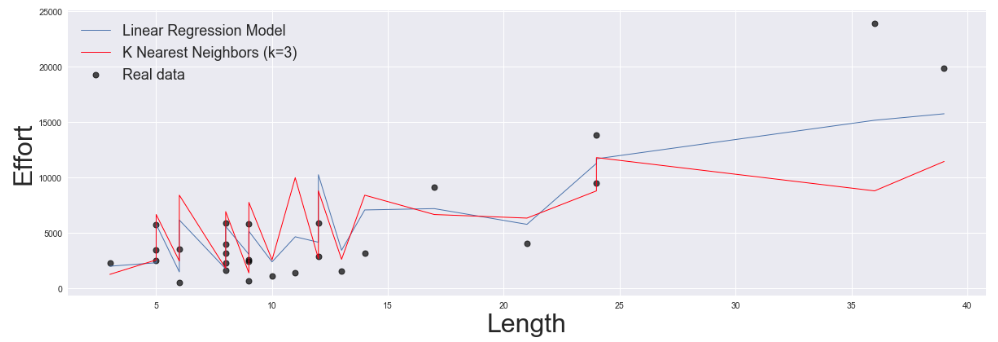
\includegraphics[height=4.6cm,width=4.6 in]{img/lenght_plot.png}
		\end{center}
	\end{block}
\end{frame}

\begin{frame}{\textit{Knn (k=3)} x \textit{LR} on Transactions Metric}
	\begin{block}{}
    It is possible to observe that the lines of both models present a slight tendency to rise, which justifies their correlation with the increase in effort.
		\begin{center}
				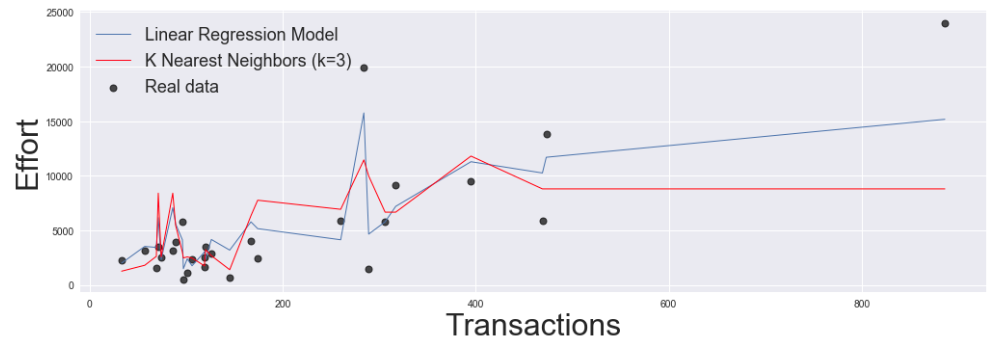
\includegraphics[height=4.7cm,width=4.6 in]{img/transactions_plot.png}
		\end{center}
	\end{block}
\end{frame}

\begin{frame}{\textit{Knn (k=3)} x \textit{LR} on Entities Metric}
Some metrics are also highlighted by the presence of outliers.
	\begin{block}{}
		\begin{center}
				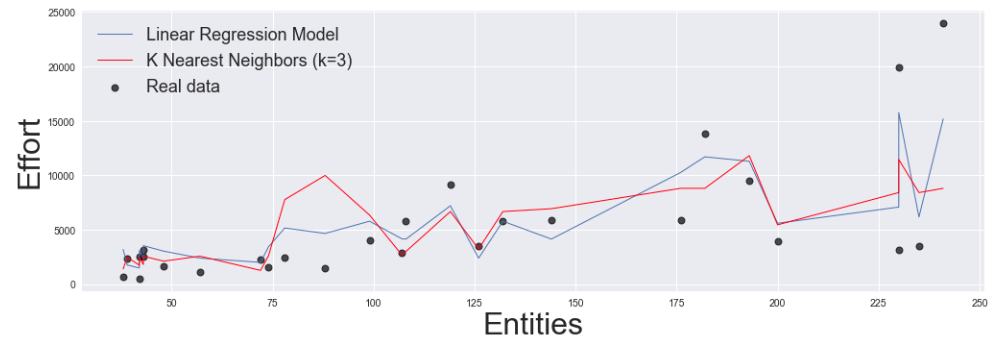
\includegraphics[height=4.7cm,width=4.6 in]{img/entities_plot.png}
		\end{center}
	\end{block}
\end{frame}

\begin{frame}{\textit{Knn (k=3)} x \textit{LR} on Points Non Adjust Metric}
	\begin{block}{}
		\begin{center}
				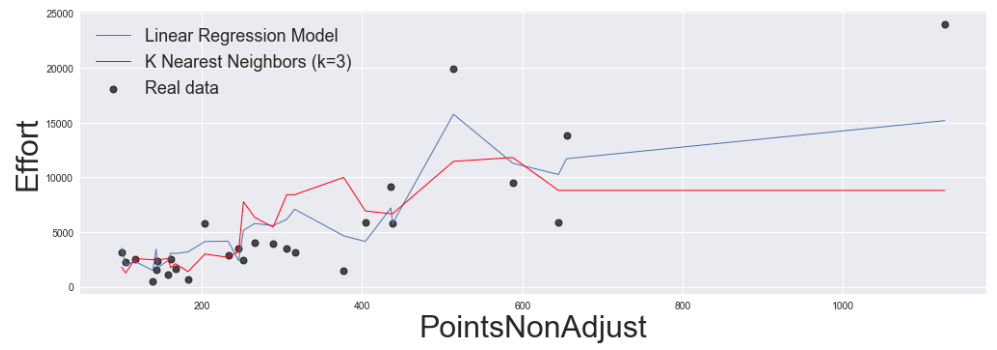
\includegraphics[height=4.7cm,width=4.6 in]{img/pointsNonAdjust_plot.png}
		\end{center}
	\end{block}
\end{frame}

\begin{frame}{\textit{Knn (k=3)} x \textit{LR} on Points Adjust Metric}
	\begin{block}{}
		\begin{center}
				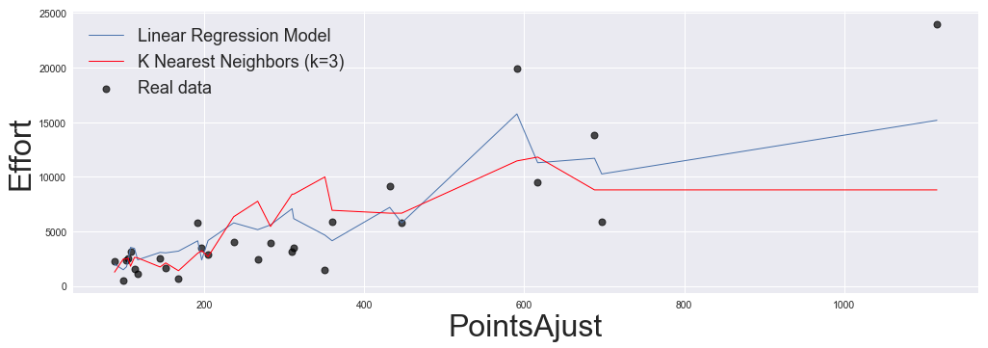
\includegraphics[height=4.7cm,width=4.6 in]{img/pointsAdjust_plot.png}
		\end{center}
	\end{block}
\end{frame}

\begin{frame}{R$^{2}$ Score Performance}
   \begin{block}{}
   
   	\begin{table}[H]
    \centering
%     \caption{Algorithms model results}
    \label{tab:modelResultsTable2}
    \smallskip
    \begin{tabular}{|l|l|}
    \hline
    \textbf{Algorithm Model} & \textbf{R$^{2}$ Score}\\[0.5ex]
    \hline
    &\\[-2ex]
    Linear Model Regression & 0.7680074954440712\\[0.5ex]
    \hline
    &\\[-2ex]
    K-Nearest Neighbor Regressor & 0.7379861869550943\\[0.5ex]
    \hline
    \end{tabular}
    \end{table}
    
    As in simple linear regression, the coefficient of determination (R$^{2}$ Score) must take values between and including 0 and 1, where the value 0 indicates that the regression is nonexistent while the value 1 indicates a "perfect" linear relationship [Freund et al. 2006].
\end{block}
\end{frame}

\section{Questions}
\begin{frame}{Questions}
	\begin{block}{Reproducible Research}
	All steps in the analytical workflow are coded in Python and available for download from a Github repository – https://github.com/toniesteves/sw-effort-predictive-analysis.information~\url{https://github.com/toniesteves/sw-effort-predictive-analysis}. 
	\end{block}
\end{frame}

\bibliographystyle{IEEEtran}
\bibliography{sigproc2,IEEEFormat}

\end{document}
	